\documentclass[tikz]{standalone}
\usepackage{amssymb}
\usepackage{amsfonts}
\usepackage{mathrsfs}
\usepackage{amsthm}
\usepackage{amsmath}
\usepackage{xcolor}
\usepackage{hyperref}
\usepackage{libertinus}
\usepackage{dsfont}
\usepackage{bm}
\usepackage{enumitem}
\usepackage{caption}
\usepackage{subcaption}
\usepackage{tikz}
\usepackage{quiver}

\newcommand{\R}{\mathbb{R}}
\newcommand{\C}{\mathbb{C}}
\newcommand{\N}{\mathbb{N}}
\newcommand{\Z}{\mathbb{Z}}
\newcommand{\Q}{\mathbb{Q}}

\newcommand{\id}{\operatorname{id}}

% differentials and derivatives
\renewcommand{\d}{\mathrm{d}}
\newcommand{\dd}{\,\d}
\newcommand{\pddf}[2]{\frac{\partial#1}{\partial#2}}
\newcommand{\ddt}{\frac{\d }{\d t}}
\newcommand{\ddtz}{\left.\ddt\right|_{t=0}}
\usetikzlibrary{arrows.meta}
\begin{document}
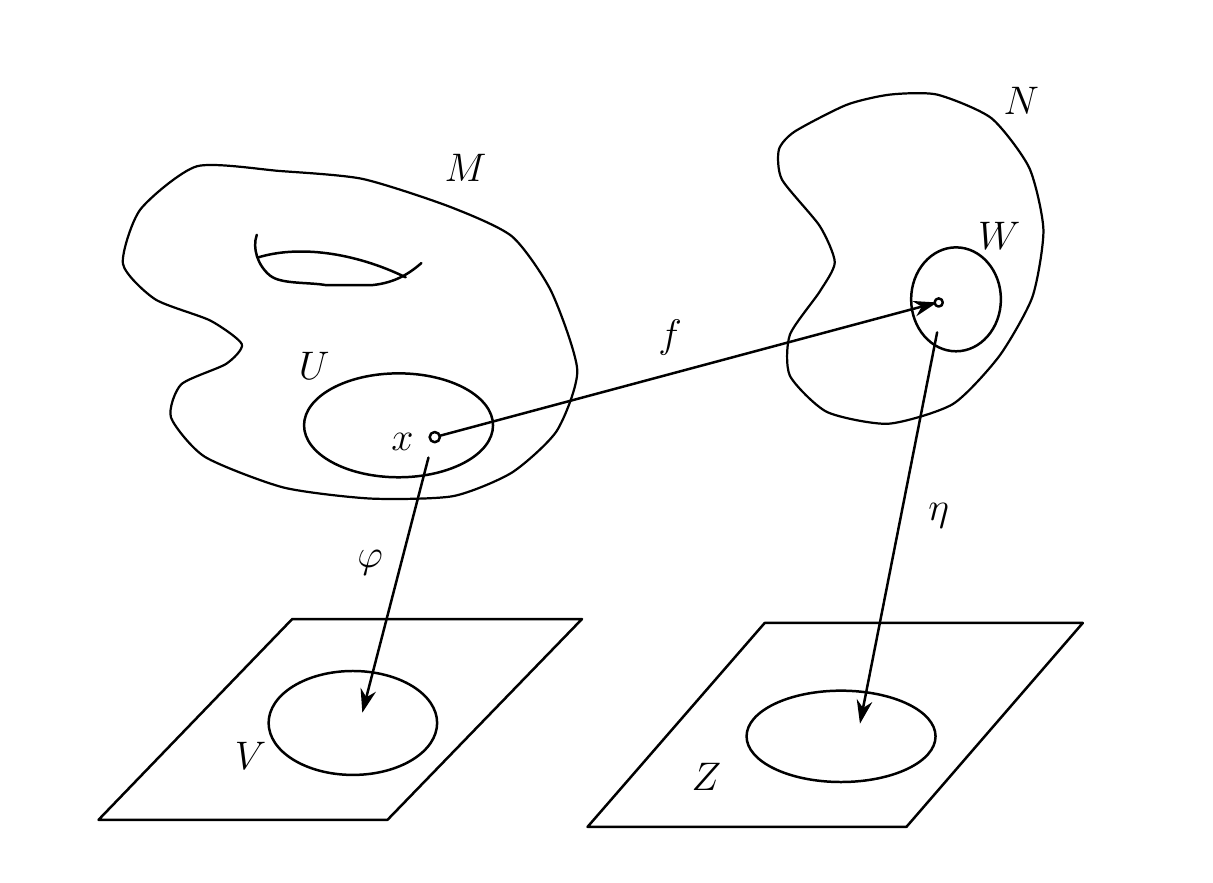
\begin{tikzpicture}[
    x=1cm, y=-1cm,
    line width=0.9pt,
    line cap=round,
    line join=round,
    >={Stealth[length=3mm,width=2mm]}
]

% Bounding box
\path[use as bounding box] (0,0) rectangle (14.7,10.5);

% ======================================
% Manifold M
% ======================================

\draw[thick]
    plot[smooth cycle, tension=0.4] coordinates {
        (1.21,3.00)
        (1.43,2.31)
        (2.15,1.76)
        (3.20,1.82)
        (4.25,1.92)
        (5.35,2.27)
        (6.15,2.65)
        (6.65,3.35)
        (6.98,4.35)
        (6.72,5.12)
        (6.15,5.65)
        (5.40,5.95)
        (4.35,5.98)
        (3.25,5.84)
        (2.25,5.45)
        (1.82,4.95)
        (1.95,4.53)
        (2.52,4.27)
        (2.72,4.02)
        (2.32,3.72)
        (1.62,3.45)
    };

\node[font=\Large] at (5.56,1.78) {$M$};

% Interior curved feature of M
\draw
    (2.91,2.63)
    .. controls (2.85,2.80) and (2.92,3.02) .. (3.08,3.15)
    .. controls (3.22,3.26) and (3.57,3.23) .. (3.79,3.27)
    -- (4.37,3.27)
    .. controls (4.68,3.24) and (4.86,3.11) .. (5.00,2.99);

\draw
    (2.92,2.92)
    .. controls (3.43,2.76) and (4.14,2.85) .. (4.80,3.17);

% Subset U
\draw (4.71,5.05) ellipse (1.20 and 0.66);
\node[font=\Large] at (3.64,4.30) {$U$};

% ======================================
% Manifold N
% ======================================

\draw[thick]
    plot[smooth cycle, tension=0.4] coordinates {
        (9.74,1.32)
        (10.40,0.98)
        (10.95,0.85)
        (11.55,0.85)
        (12.24,1.15)
        (12.72,1.78)
        (12.90,2.57)
        (12.76,3.42)
        (12.34,4.17)
        (11.75,4.78)
        (10.93,5.03)
        (10.15,4.88)
        (9.68,4.42)
        (9.68,3.90)
        (10.06,3.35)
        (10.25,2.98)
        (10.06,2.52)
        (9.58,1.93)
        (9.54,1.55)
    };

\node[font=\Large] at (12.62,0.93) {$N$};

% Subset W
\draw (11.79,3.45) ellipse (0.57 and 0.66);
\node[font=\Large] at (12.34,2.65) {$W$};

% ======================================
% Lower spaces
% ======================================

% Left plane
\draw
    (0.90,10.06) --
    (4.57,10.06) --
    (7.04,7.51) --
    (3.36,7.51) -- cycle;

% Subset V
\draw (4.13,8.83) ellipse (1.07 and 0.66);
\node[font=\Large] at (2.83,9.25) {$V$};

% Right plane
\draw
    (7.11,10.15) --
    (11.16,10.15) --
    (13.40,7.56) --
    (9.36,7.56) -- cycle;

% Subset Z
\draw (10.33,9.00) ellipse (1.20 and 0.58);
\node[font=\Large] at (8.62,9.52) {$Z$};

% ======================================
% Maps
% ======================================

% Map F: M -> N
\draw[->] (5.17,5.20) -- (11.55,3.49);
\node[font=\Large] at (8.16,3.94) {$f$};

% Map phi
\draw[->] (5.09,5.46) -- (4.25,8.70);
\node[font=\Large] at (4.35,6.79) {$\varphi$};

% Map eta
\draw[->] (11.55,3.87) -- (10.57,8.84);
\node[font=\Large] at (11.57,6.20) {$\eta$};

% ======================================
% Distinguished points
% ======================================

% Point x in U
\fill[white] (5.17,5.20) circle (0.065);
\draw (5.17,5.20) circle (0.065);
\node[font=\Large] at (4.76,5.26) {$x$};

% Image F(x) in W
\fill[white] (11.57,3.49) circle (0.052);
\draw (11.57,3.49) circle (0.052);

\end{tikzpicture}

\end{document}